\documentclass[12pt,a4paper]{article}
\usepackage[utf8]{inputenc}
\usepackage[T1]{fontenc}
\usepackage[brazil]{babel}
\usepackage{lmodern,graphicx,xcolor,geometry,fancyhdr,hyperref}
\geometry{left=2cm,right=2cm,top=2cm,bottom=1.8cm,headheight=14pt}
\definecolor{navy}{HTML}{173544}\definecolor{teal}{HTML}{087F8C}
\hypersetup{colorlinks=true,urlcolor=teal,linkcolor=navy,pdftitle={Roteiro detalhado do pitch - ENEM 2023},pdfauthor={Joey Alan de Freitas Solis; Paulo Henrico}}
\setlength{\parindent}{0pt}\setlength{\parskip}{4pt}
\pagestyle{fancy}\fancyhf{}\fancyhead[L]{\small ENEM 2023 | Roteiro do apresentador}\fancyhead[R]{\small 23 slides finais}\fancyfoot[R]{\thepage}
\newcommand{\rotulo}[1]{\par\vspace{3pt}{\color{teal}\bfseries #1}\par\nopagebreak}
\begin{document}
\thispagestyle{empty}
\vspace*{2cm}
{\color{teal}\Large APRESENTAÇÃO E DEFESA DO PROJETO}\par\vspace{1cm}
{\color{navy}\Huge\bfseries ENEM 2023}\par\vspace{0.5cm}
{\color{navy}\LARGE Roteiro detalhado do pitch}\par\vspace{0.6cm}
{\large Comparação nacional de dez regressores e da referência pela média}\par
\vspace{1cm}
Joey Alan de Freitas Solis e Paulo Henrico\\
Universidade de Fortaleza (Unifor)\\Professor Tulio
\vspace{1cm}
\rotulo{Como usar}
Este roteiro acompanha, na mesma ordem, os 23 slides finais do Canva. As miniaturas são referências visuais; a numeração atual aparece no título de cada página. Cada slide tem uma fala principal, explicação de apoio, orientação para ler o visual, uma pergunta de defesa e uma transição. A explicação de apoio serve para estudar e responder à banca; não precisa ser lida integralmente no pitch.
\rotulo{Versão de referência}
Apresentação ampliada em 16 de novembro de 2026. O catálogo completo está no slide 7, os modelos independentes nos slides 8 a 10, o ranking no slide 13 e o teste final no slide 19. Os valores são resultados registrados do projeto; nenhum experimento novo foi feito para produzir este roteiro.
\href{https://www.canva.com/design/DAHbBYEq0BQ/NpBSvagoxA2EQUM0qQ8hSg/edit}{Abrir a apresentação final no Canva}
\rotulo{Planejamento de tempo}
Para uma exposição detalhada, reservar aproximadamente 15 a 20 minutos para a fala principal e ajustar após ensaio. Se o limite for 12 minutos, resumir as explicações e usar os aprofundamentos apenas nas perguntas. Os tempos são sugestões, não duração medida.
\clearpage
{\color{navy}\LARGE\bfseries Mapa da apresentação}\par\vspace{0.5cm}
\rotulo{Joey: slides 1 a 10}
Contexto e pergunta; origem e divisão dos dados; atributos; preparação; três dobras; catálogo completo; linear, Ridge e árvore isolada.
\rotulo{Paulo: slides 11 a 23}
Stacking e suas dobras internas; métricas e ranking; engenharia; seleção e PCA; ponderação e ablações; buscas; curvas; teste final; erros e grupos; limites e conclusão.
\rotulo{Quatro distinções para manter claras}
1. NU\_NOTA\_CN é o alvo; Q005 é quantidade de moradores e entra como atributo numérico.\\
2. Treino e validação pertencem ao desenvolvimento; o teste de 20\% é separado e já foi avaliado após congelar as receitas.\\
3. O trio geral é Stacking, Ridge e linear. Stacking, SVM e floresta são o trio do recorte de sete.\\
4. Testes de software, avaliações por dobra e pontos de curva são evidências diferentes. Não devem ser contados como treinamentos novos equivalentes.
\rotulo{Vocabulário para a fala}
\textbf{Ajuste}: aprender parâmetros usando treino. \textbf{Hiperparâmetro}: configuração escolhida antes do ajuste. \textbf{Validação}: dados separados para comparar alternativas no desenvolvimento. \textbf{Teste final}: avaliação da receita congelada. \textbf{Resíduo}: nota observada menos prevista. \textbf{Generalização}: desempenho em dados não usados no ajuste.
\rotulo{Valores de referência para conferir durante o ensaio}
Base original: 3.933.955 registros. Elegíveis: 2.692.427. Desenvolvimento: 2.153.941. Teste: 538.486. Entradas originais: 40. Semente: 42. Dobras externas: 3. Stacking no teste: RMSE 76,190; MAE 55,325; R\textsuperscript{2} 0,2497. Ganho de RMSE contra a média: 13,38\%. Diferença contra linear: 0,327 ponto.
\rotulo{Fontes para conferir uma resposta}
Configuração: \texttt{configs/ciencias\_natureza.toml}\\
Métricas: \texttt{resultados/comparacao\_modelos.csv}\\
Tabelas adicionais: \texttt{resultados/tabelas/}\\
Artigo: \texttt{docs/artigo.pdf}\\
Modelos: \texttt{src/enem\_base/modeling.py}\\
Os caminhos são relativos à raiz do repositório.

\clearpage
{\color{teal}\small SLIDE 1 / 23 - JOEY}\par
{\color{navy}\Large\bfseries Predição da nota de Ciências da Natureza}\par
{\small Abertura e proposta}\par
\begin{center}
\includegraphics[height=3.5cm,trim=0 26.88bp 0 0,clip]{figuras/roteiro/slide-01.png}\end{center}
\rotulo{Fala principal sugerida}
Nosso trabalho compara dez regressores e uma referência pela média para estimar a nota de Ciências da Natureza no ENEM 2023. Usamos registros reais de participantes de todo o Brasil e mantivemos as mesmas partições para comparar os modelos. O objetivo foi verificar o desempenho e compreender os limites das previsões. O principal resultado foi o menor RMSE do Stacking, com vantagem pequena sobre uma regressão linear simples.
\rotulo{Explicação para estudar e aprofundar}
Apresente os autores e o contexto acadêmico na Unifor. Explique que nacional significa cobertura dos participantes elegíveis desta edição, não uma amostra representativa de toda a população brasileira. O diferencial demonstrado é a comparação consistente em escala nacional, acompanhada de resultados negativos e análise dos erros. O projeto é um estudo acadêmico exploratório; não valida uma ferramenta para tomar decisões individuais sobre estudantes.
\rotulo{Como explicar o visual}
Use a capa para situar o tema. Não antecipe todos os números: destaque apenas tarefa, comparação justa e leitura crítica.
\rotulo{Pergunta provável e resposta}
O projeto prevê aprovação no ENEM? Não. Ele estima uma nota numérica de Ciências da Natureza, sem definir aprovação ou classificar pessoas.
\rotulo{Transição}
Primeiro, precisamos delimitar a pergunta que esses modelos tentam responder.
\vfill{\raggedright\scriptsize\color{navy} Conferência no projeto: README.md; configs/ciencias\_natureza.toml.}\par
\clearpage
{\color{teal}\small SLIDE 2 / 23 - JOEY}\par
{\color{navy}\Large\bfseries Pergunta de pesquisa e objetivos}\par
{\small Problema, objetivo e utilidade}\par
\begin{center}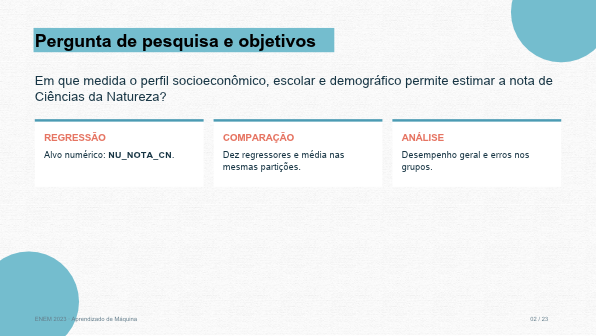
\includegraphics[height=3.5cm,trim=0 26.88bp 0 0,clip]{figuras/roteiro/slide-02.png}\end{center}
\rotulo{Fala principal sugerida}
Queremos saber em que medida o perfil socioeconômico, escolar e demográfico permite estimar uma nota de Ciências da Natureza. Como a saída é um número, trabalhamos com regressão. Comparamos os erros dos algoritmos e investigamos em quais grupos ou faixas de nota eles erram mais. Isso ajuda a avaliar o quanto essas informações descrevem o desempenho observado, sem atribuir uma causa à renda, à escola ou a outra característica.
\rotulo{Explicação para estudar e aprofundar}
Regressão supervisionada utiliza exemplos com entradas e uma saída conhecida. Durante o treino, o modelo ajusta seus parâmetros para aproximar essa saída. Depois, comparamos previsões e notas reais em registros separados. Associação preditiva não é causalidade: um atributo pode ajudar a prever por estar associado a outras condições não observadas. A utilidade demonstrada é metodológica e descritiva, adequada ao debate acadêmico sobre previsibilidade e limitações dos dados.
\rotulo{Como explicar o visual}
Percorra os três blocos: alvo contínuo, comparação nas mesmas partições e diagnóstico dos erros. A pergunta de pesquisa conecta todo o pitch.
\rotulo{Pergunta provável e resposta}
Por que não é classificação? Porque não criamos rótulos como aprovado ou reprovado; o valor previsto continua sendo uma nota.
\rotulo{Transição}
Para responder à pergunta, começamos pela origem e pela qualidade dos dados.
\vfill{\raggedright\scriptsize\color{navy} Conferência no projeto: configs/ciencias\_natureza.toml; docs/artigo.md.}\par
\clearpage
{\color{teal}\small SLIDE 3 / 23 - JOEY}\par
{\color{navy}\Large\bfseries População e divisão dos dados}\par
{\small Fonte e população efetivamente utilizada}\par
\begin{center}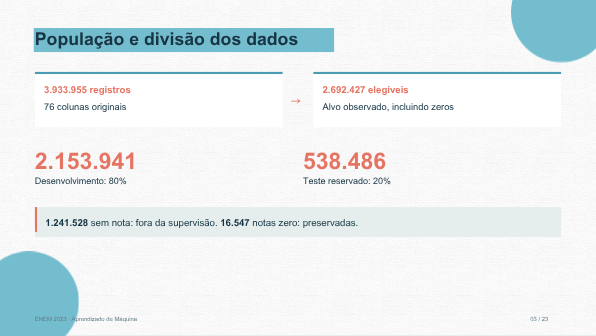
\includegraphics[height=3.5cm,trim=0 26.88bp 0 0,clip]{figuras/roteiro/slide-03.png}\end{center}
\rotulo{Fala principal sugerida}
A base original contém 3.933.955 registros e 76 colunas. Para treinar uma regressão supervisionada, precisamos conhecer a nota real: 2.692.427 participantes tinham Ciências da Natureza observada. Os 1.241.528 sem essa nota ficaram fora da supervisão. Isso é diferente de nota zero: os 16.547 zeros observados foram mantidos. Dividimos os elegíveis em 2.153.941 para desenvolvimento e 538.486 para teste.
\rotulo{Explicação para estudar e aprofundar}
A importação foi feita em lotes, normalizando espaços, tokens de ausência e tipos, sem editar os arquivos originais. O projeto registrou integridade dos ZIPs e hashes e confirmou a igualdade do CSV normalizado com os Parquets preparados. Não houve substituição por dados sintéticos no experimento nacional. Fixtures fictícias pertencem apenas aos testes de software. O complemento de competências de redação foi preservado, mas não foi integrado aos preditores desta tarefa.
\rotulo{Como explicar o visual}
Aponte a passagem de base original para elegíveis e depois os dois conjuntos. Explique por que excluir alvo ausente não significa apagar a pessoa da importação original.
\rotulo{Pergunta provável e resposta}
Foi imputada uma nota para quem não fez a prova? Não. O alvo ausente não foi preenchido nem convertido em zero.
\rotulo{Transição}
Com a população definida, precisamos mostrar quais informações os modelos receberam.
\vfill{\raggedright\scriptsize\color{navy} Conferência no projeto: src/enem\_base/ingestion.py; src/enem\_base/cleaning.py; dados/raw/README.md.}\par
\clearpage
{\color{teal}\small SLIDE 4 / 23 - JOEY}\par
{\color{navy}\Large\bfseries 40 atributos originais de perfil}\par
{\small Entradas, alvo e identificador}\par
\begin{center}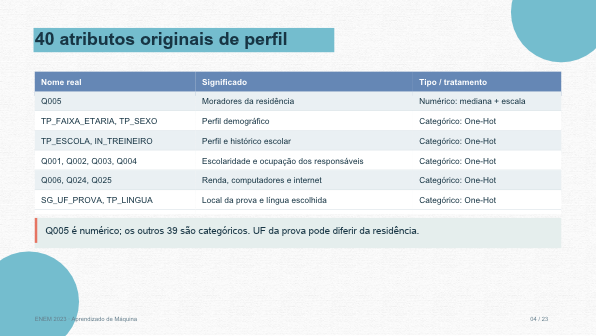
\includegraphics[height=3.5cm,trim=0 26.88bp 0 0,clip]{figuras/roteiro/slide-04.png}\end{center}
\rotulo{Fala principal sugerida}
Utilizamos quarenta atributos originais. Q005 representa o número de moradores e é a única entrada numérica original; os outros trinta e nove atributos são tratados como categóricos. Há dados demográficos, escolares e do questionário socioeconômico. O alvo é NU\_NOTA\_CN. O identificador NU\_INSCRICAO serve para controlar participantes e partições, sem entrar no modelo. Também não usamos outras notas, respostas, gabaritos ou presença como preditores.
\rotulo{Explicação para estudar e aprofundar}
Não confunda Q005 com o alvo: quantidade de moradores é uma entrada; a nota de Ciências da Natureza é a saída que tentamos estimar. Códigos numéricos de categorias não significam necessariamente quantidades ou distâncias. Por isso, renda Q006 e escolaridade Q001/Q002 recebem codificação categórica na receita original. SG\_UF\_PROVA indica a UF de aplicação, que pode ser diferente da residência. A lista completa das quarenta entradas está na configuração e no guia de fala.
\rotulo{Como explicar o visual}
Leia exemplos da tabela, evitando recitar os quarenta nomes. Relacione nome real, significado e tratamento. Destaque a diferença entre entrada e alvo.
\rotulo{Pergunta provável e resposta}
Todas as entradas se tornam binárias? Não. As categorias viram indicadores, mas Q005 continua numérica e é padronizada.
\rotulo{Transição}
Antes de treinar, essas entradas precisam de uma representação que evite vazamento.
\vfill{\raggedright\scriptsize\color{navy} Conferência no projeto: configs/ciencias\_natureza.toml: seção features; resultados/colunas.csv.}\par
\clearpage
{\color{teal}\small SLIDE 5 / 23 - JOEY}\par
{\color{navy}\Large\bfseries Pré-processamento e prevenção de vazamento}\par
{\small Limpeza e prevenção de vazamento}\par
\begin{center}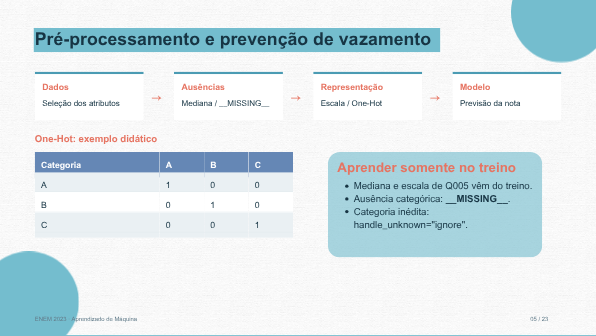
\includegraphics[height=3.5cm,trim=0 26.88bp 0 0,clip]{figuras/roteiro/slide-05.png}\end{center}
\rotulo{Fala principal sugerida}
A limpeza de formato acontece na importação; a preparação estatística acontece dentro de cada treino. Q005 recebe a mediana quando necessário e passa por padronização. Nas categorias, a ausência recebe um marcador próprio e a codificação one-hot cria indicadores de categoria. Mediana, escala e categorias aprendidas não são ajustadas usando a validação ou o teste. Esse isolamento impede que a preparação antecipe informações da avaliação.
\rotulo{Explicação para estudar e aprofundar}
Vazamento ocorre quando uma decisão de treino utiliza informação que deveria estar fora dele. Calcular a média ou a mediana na base inteira antes de separar as dobras já quebraria esse isolamento. O Pipeline organiza preparação e regressor no mesmo ajuste. No one-hot, uma categoria A pode virar 1,0,0 e B virar 0,1,0: é um exemplo didático de representação, não uma previsão. Categorias inéditas são ignoradas pelo codificador; desconhecimento previsto no dicionário permanece distinto de ausência. O indicador de ausência numérica é criado quando aplicável.
\rotulo{Como explicar o visual}
Mostre o fluxo e a pequena tabela A/B/C. Aqui A/B/C são categorias didáticas; no próximo slide as mesmas letras representarão partes dos participantes.
\rotulo{Pergunta provável e resposta}
Padronizar muda a informação? Muda a escala numérica, usando parâmetros do treino; não cria novas notas nem transforma Q005 em categoria.
\rotulo{Transição}
Agora veremos quais participantes entram no treino e na validação em cada rodada.
\vfill{\raggedright\scriptsize\color{navy} Conferência no projeto: src/enem\_base/preprocessing.py: build\_preprocessor; src/enem\_base/modeling.py: pipeline.}\par
\clearpage
{\color{teal}\small SLIDE 6 / 23 - JOEY}\par
{\color{navy}\Large\bfseries Três dobras com o teste reservado}\par
{\small Dobras, divisão e semente}\par
\begin{center}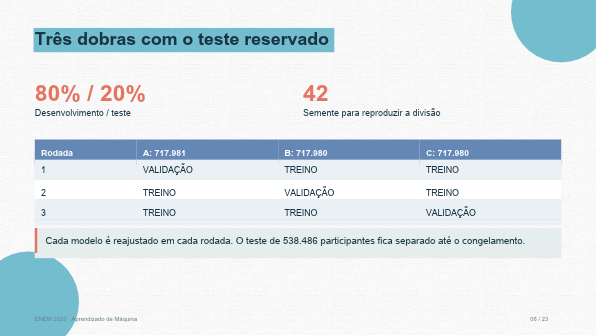
\includegraphics[height=3.5cm,trim=0 26.88bp 0 0,clip]{figuras/roteiro/slide-06.png}\end{center}
\rotulo{Fala principal sugerida}
Separamos 80\% dos elegíveis para desenvolvimento e 20\% para o teste final. Dentro do desenvolvimento, criamos três partes fixas: A, B e C. Na primeira rodada, treinamos em B e C e validamos em A. Na segunda, treinamos em A e C e validamos em B. Na terceira, treinamos em A e B e validamos em C. Assim, cada participante do desenvolvimento é avaliado uma vez fora do treino daquele ajuste.
\rotulo{Explicação para estudar e aprofundar}
A tem 717.981 participantes; B e C têm 717.980 cada. Os treinos têm 1.435.960 ou 1.435.961 pessoas. Cada rodada reajusta o modelo e sua preparação. As dobras são as mesmas para todos os algoritmos. A semente 42 controla o sorteio para reproduzir a divisão com os mesmos dados e configuração; não melhora automaticamente o resultado. O teste ficou fora das escolhas, foi usado após o congelamento das receitas e já foi concluído. Três dobras externas não são três testes finais.
\rotulo{Como explicar o visual}
Leia cada linha da matriz, mostrando duas células de treino e uma de validação. A cor identifica o papel da parte naquela rodada.
\rotulo{Pergunta provável e resposta}
O teste é a terceira dobra? Não. Ele foi separado antes; as três dobras pertencem somente aos 80\% do desenvolvimento.
\rotulo{Transição}
Com esse protocolo comum, podemos comparar os mecanismos de aprendizagem.
\vfill{\raggedright\scriptsize\color{navy} Conferência no projeto: src/enem\_base/splits.py: save\_splits; dados/splits/README.md.}\par
\clearpage
{\color{teal}\small SLIDE 7 / 23 - JOEY}\par
{\color{navy}\Large\bfseries Dez regressores efetivamente avaliados}\par
{\small Algoritmos e escolhas práticas}\par
\begin{center}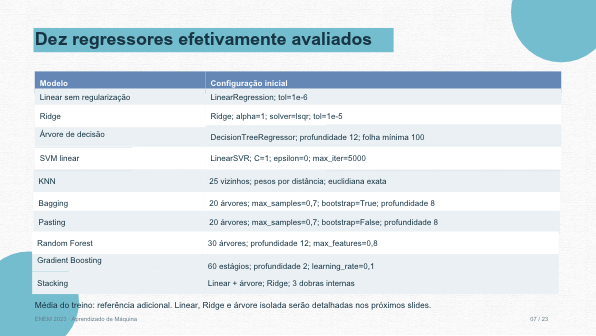
\includegraphics[height=3.5cm,trim=0 26.88bp 0 0,clip]{figuras/roteiro/slide-07.png}\end{center}
\rotulo{Fala principal sugerida}
A tabela reúne todos os dez regressores executados: linear sem regularização, Ridge, árvore de decisão, SVM linear, KNN, Bagging, Pasting, Random Forest, Gradient Boosting e Stacking. A média do treino é uma referência adicional. Todos usam as mesmas três dobras e o mesmo critério principal. Os próximos slides detalham linear, Ridge e árvore isolada, que antes estavam apenas numa observação.
\rotulo{Explicação para estudar e aprofundar}
Ridge atende à opção de regressão linear com regularização; não é obrigatório acrescentar Lasso. LinearSVR é permitido no enunciado. A escolha linear define uma hipótese aditiva e uma implementação viável para este protocolo nacional, mas não demonstra superioridade sobre RBF ou polinomial, que não foram comparados. GradientBoostingRegressor atende à exigência de ao menos um boosting; AdaBoost, XGBoost e outros não foram executados. O KNN real é ExactProfileKNeighborsRegressor, uma implementação própria de regressão com 25 vizinhos e busca euclidiana exata, não uma instância literal de KNeighborsRegressor. Faiss não transforma a busca em aproximação. Bagging e Pasting usam vinte árvores e 70\% do treino, com e sem reposição. Random Forest obteve RMSE 76,643 contra 77,484 do Bagging; também mudam quantidade e profundidade das árvores, portanto não isolamos o efeito do sorteio de atributos. A folha mínima é cem nas árvores. As configurações iniciais não foram alteradas nesta revisão.
\rotulo{Como explicar o visual}
Explique os mecanismos em pares: Bagging/Pasting e Random Forest/Boosting. A tabela mostra configurações iniciais; a busca de parâmetros aparece depois.
\rotulo{Pergunta provável e resposta}
A lista está completa? Sim: há dez regressores, incluindo a linear com e sem regularização e a árvore isolada, mais o baseline. As alternativas não executadas não devem ser apresentadas como modelos testados.
\rotulo{Transição}
Começamos pelos três regressores que faltavam na explicação individual, a partir da linear sem regularização.
\vfill{\raggedright\scriptsize\color{navy} Conferência no projeto: src/enem\_base/modeling.py: model\_catalog; src/enem\_base/neighbors.py.}\par
\clearpage
{\color{teal}\small SLIDE 8 / 23 - JOEY}\par
{\color{navy}\Large\bfseries Linear sem regularização}\par
{\small Modelo de referência e base do Stacking}\par
\begin{center}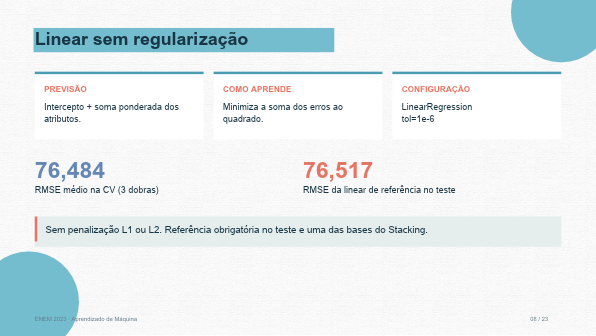
\includegraphics[height=3.5cm,trim=0 26.88bp 0 0,clip]{figuras/roteiro/slide-08.png}\end{center}
\rotulo{Fala principal sugerida}
A regressão linear sem regularização estima a nota por um intercepto somado aos atributos multiplicados por coeficientes aprendidos. O ajuste minimiza a soma dos erros ao quadrado, sem uma penalização L1 ou L2. Essa é uma referência importante: antes de defender um ensemble, precisamos verificar se ele supera uma solução simples. A linear teve RMSE médio de 76,484 na validação e 76,517 no teste final.
\rotulo{Explicação para estudar e aprofundar}
A fórmula geral é nota prevista = intercepto + soma dos coeficientes vezes as entradas preparadas. Os indicadores one-hot permitem coeficientes diferentes para categorias, enquanto Q005 permanece numérica padronizada. Os coeficientes são aprendidos no treino; não foram publicados nos slides como uma equação numérica final. Tol=1e-6 é a tolerância inicial do solucionador, não uma penalização de regularização. A linear usa o mesmo Pipeline e as mesmas dobras dos outros modelos. Ela também é uma base do Stacking, mas sua avaliação isolada é um experimento distinto. Na busca foi selecionado tol=1e-5; a referência do teste conserva tol=1e-6. Coeficientes preditivos não identificam efeitos causais.
\rotulo{Como explicar o visual}
Percorra previsão, ajuste e configuração. Compare os dois números com cuidado: o primeiro resume três dobras; o segundo pertence ao teste final, em outro conjunto de participantes.
\rotulo{Pergunta provável e resposta}
Sem regularização significa sem preparação? Não. A linear recebe a mesma preparação das entradas; o que não existe é a penalização adicional L1 ou L2 nos coeficientes.
\rotulo{Transição}
Agora veremos uma regressão linear que acrescenta controle sobre o tamanho dos coeficientes: Ridge.
\rotulo{Referência técnica}
\href{https://scikit-learn.org/stable/modules/generated/sklearn.linear_model.LinearRegression.html}{Documentação oficial do scikit-learn}
\vfill{\scriptsize\color{navy} Conferência: src/enem\_base/modeling.py: model\_catalog;\\ resultados/comparacao\_modelos.csv;\\ resultados/tabelas/comparacao\_teste.csv.}\par
\clearpage
{\color{teal}\small SLIDE 9 / 23 - JOEY}\par
{\color{navy}\Large\bfseries Ridge: regularização L2}\par
{\small Regressor independente com penalização dos coeficientes}\par
\begin{center}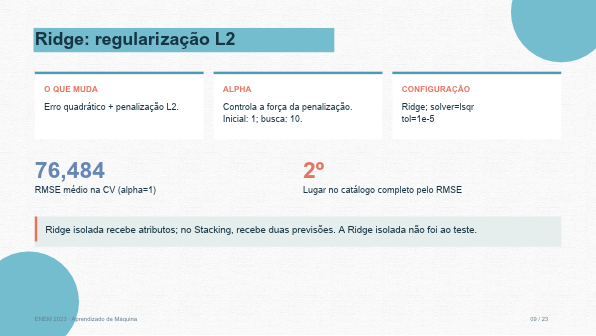
\includegraphics[height=3.5cm,trim=0 26.88bp 0 0,clip]{figuras/roteiro/slide-09.png}\end{center}
\rotulo{Fala principal sugerida}
Ridge também aprende uma combinação linear dos atributos, mas acrescenta uma penalização L2. O objetivo combina a soma dos erros quadráticos com alpha vezes a soma dos coeficientes ao quadrado. Alpha controla a força dessa penalização. Como regressor independente, Ridge recebe as quarenta entradas originais após preparação, e não as previsões de outros modelos. Seu RMSE inicial foi 76,484, com a segunda colocação no ranking completo antes do arredondamento.
\rotulo{Explicação para estudar e aprofundar}
A penalização desencoraja coeficientes muito grandes e permite controlar a complexidade. Isso pode ajudar quando há entradas correlacionadas, mas não garante menor erro em qualquer base. A receita inicial tem alpha=1, solver=lsqr e tol=1e-5. A busca selecionou alpha=10, com ganho de aproximadamente 0,0000376 ponto de RMSE. O RMSE inicial exato foi 76,483610, contra 76,483799 da linear: ambos aparecem como 76,484 nos slides. A diferença é muito pequena e não recebeu teste de significância. Há dois usos distintos de Ridge: isolada, aprende dos atributos; como combinador do Stacking, aprende das duas previsões OOF. No combinador, alpha passou de 1 para 1000. A Ridge isolada tem CV completa, mas não foi avaliada no teste final deste protocolo. Lasso seria uma alternativa permitida de regularização; não foi o método executado.
\rotulo{Como explicar o visual}
Explique o que muda na função de ajuste e o significado de alpha. A posição de segundo lugar é pelo RMSE da CV inicial, não pelo teste. O número grande é o RMSE inicial, não o valor de alpha.
\rotulo{Pergunta provável e resposta}
Ridge é apenas uma etapa do Stacking? Não. O projeto avaliou uma Ridge independente e também utiliza outra Ridge como combinador, com entradas e configurações diferentes.
\rotulo{Transição}
A seguir, saímos da combinação linear para um modelo que aprende regras: a árvore de decisão.
\rotulo{Referência técnica}
\href{https://scikit-learn.org/stable/modules/generated/sklearn.linear_model.Ridge.html}{Documentação oficial do scikit-learn}
\vfill{\scriptsize\color{navy} Conferência: src/enem\_base/modeling.py: model\_catalog;\\ src/enem\_base/tuning.py: SPACES;\\ resultados/comparacao\_modelos.csv.}\par
\clearpage
{\color{teal}\small SLIDE 10 / 23 - JOEY}\par
{\color{navy}\Large\bfseries Árvore de decisão isolada}\par
{\small Regras de divisão e previsão pela média de uma folha}\par
\begin{center}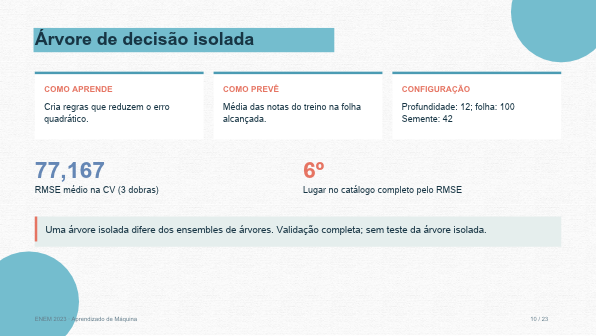
\includegraphics[height=3.5cm,trim=0 26.88bp 0 0,clip]{figuras/roteiro/slide-10.png}\end{center}
\rotulo{Fala principal sugerida}
A árvore de decisão aprende regras sobre os atributos preparados e divide o treino em regiões. Em cada divisão, busca reduzir o erro quadrático. Para uma nova pessoa, percorremos as regras até uma folha, e a previsão é a média das notas do treino naquela folha. A árvore isolada teve RMSE médio de 77,167 e ficou em sexto no catálogo completo. Ela é um modelo próprio e também uma das bases do Stacking.
\rotulo{Explicação para estudar e aprofundar}
Foi utilizado DecisionTreeRegressor, com profundidade máxima doze, pelo menos cem participantes em cada folha e semente 42. O critério padrão squared\_error corresponde à redução da variância dentro das regiões e à previsão pela média da folha. Profundidade doze não significa doze árvores, e folha mínima cem não significa cem folhas. Esses limites restringem a complexidade de uma árvore que, sem controles, pode ajustar detalhes particulares do treino. A árvore permite relações não lineares e interações entre entradas, sem aprender uma única soma linear global. Sua preparação continua restrita ao treino da dobra. Bagging, Pasting, floresta e boosting combinam várias árvores; não devem ser confundidos com este estimador isolado. Os experimentos com PCA também incluíram a árvore, mas a variante não melhorou o RMSE. Não há previsão da árvore isolada no teste final.
\rotulo{Como explicar o visual}
Leia as três etapas: aprender regras, prever pela média e controlar complexidade. Os números destacam erro de validação e posição no ranking, sem representar uma avaliação final no teste.
\rotulo{Pergunta provável e resposta}
Por que Random Forest pode diferir da árvore? A floresta agrega árvores com aleatoriedade e média de previsões. As configurações também diferem; a comparação observada não isola um único efeito.
\rotulo{Transição}
Com linear, Ridge e árvore isolada esclarecidas, podemos entender como duas dessas bases são combinadas no Stacking.
\rotulo{Referência técnica}
\href{https://scikit-learn.org/stable/modules/generated/sklearn.tree.DecisionTreeRegressor.html}{Documentação oficial do scikit-learn}
\vfill{\scriptsize\color{navy} Conferência: src/enem\_base/modeling.py: DecisionTreeRegressor;\\ resultados/comparacao\_modelos.csv.}\par
\clearpage
{\color{teal}\small SLIDE 11 / 23 - PAULO}\par
{\color{navy}\Large\bfseries Stacking: duas bases e um combinador}\par
{\small Stacking, previsões OOF e Ridge}\par
\begin{center}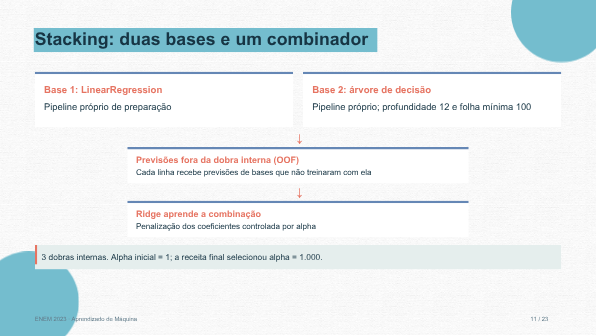
\includegraphics[height=3.5cm,trim=0 26.88bp 0 0,clip]{figuras/roteiro/slide-11.png}\end{center}
\rotulo{Fala principal sugerida}
Nosso Stacking tem duas bases: regressão linear e árvore de decisão. Primeiro, produz previsões internas para participantes que não estavam no treino da base naquela rodada. Essas previsões fora da dobra, chamadas OOF, tornam-se entradas de uma regressão Ridge que aprende a combinação. Portanto, o combinador aprende com erros de generalização das bases, em vez de receber apenas previsões sobre pessoas que elas já conheceram.
\rotulo{Explicação para estudar e aprofundar}
As três dobras internas servem para treinar o combinador; as três externas servem para avaliar o Stacking inteiro. Cada base possui seu próprio Pipeline, inclusive nas dobras internas. Ridge é regressão linear com penalização L2: minimiza o erro quadrático junto de uma penalização para coeficientes grandes. Alpha controla sua força. A receita inicial usa alpha=1 e a final usa 1000, com ganho de busca de apenas cerca de 3,205 vezes 10 elevado a menos 8 ponto de RMSE. SVM e Random Forest não são bases deste Stacking. Os coeficientes numéricos da combinação não são exibidos nos slides.
\rotulo{Como explicar o visual}
Siga o diagrama de cima para baixo: duas bases, previsões OOF e combinador Ridge. Não confunda combinação aprendida com média simples fixa.
\rotulo{Pergunta provável e resposta}
Qual é a fórmula? Ela combina linearmente as duas previsões com coeficientes aprendidos. Não há valores de coeficientes publicados no slide para apresentar como fórmula numérica final.
\rotulo{Transição}
Para julgar se essa combinação ajuda, precisamos definir o significado das métricas.
\vfill{\raggedright\scriptsize\color{navy} Conferência no projeto: src/enem\_base/modeling.py: StackingRegressor; src/enem\_base/tuning.py: ALPHAS.}\par
\clearpage
{\color{teal}\small SLIDE 12 / 23 - PAULO}\par
{\color{navy}\Large\bfseries Métricas e modelos de referência}\par
{\small Como explicar RMSE, MAE e R\textsuperscript{2}}\par
\begin{center}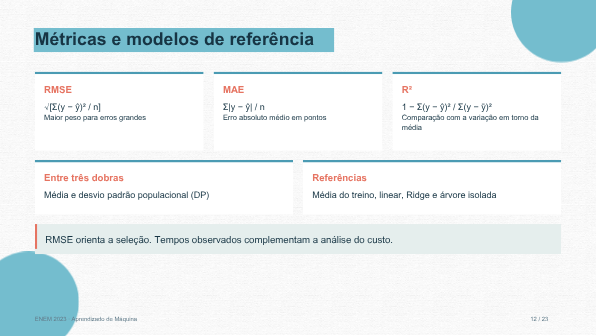
\includegraphics[height=3.5cm,trim=0 26.88bp 0 0,clip]{figuras/roteiro/slide-12.png}\end{center}
\rotulo{Fala principal sugerida}
O RMSE é a raiz da média dos erros ao quadrado, em pontos da nota. Ele dá maior peso a erros grandes e é nosso critério principal. O MAE é a média dos erros absolutos, também em pontos. O R\textsuperscript{2} compara o erro quadrático com a variação em torno da média observada. RMSE e MAE menores são melhores; R\textsuperscript{2} maior é melhor. Resumimos a validação pela média e pelo desvio padrão das três dobras.
\rotulo{Explicação para estudar e aprofundar}
Nas fórmulas, y é a nota real, y previsto é a estimativa e n é o total avaliado. Como exemplo didático, erros de dez e trinta pontos produzem MAE de vinte e RMSE de aproximadamente 22,36; isso ilustra a penalização dos erros maiores, sem representar resultados do projeto. O desvio padrão populacional entre três dobras descreve variação e não é intervalo de confiança. O baseline prevê a média do alvo do treino, sem usar atributos. Um R\textsuperscript{2} perto de 0,25 não significa 25\% de acertos nem prova sozinho subajuste.
\rotulo{Como explicar o visual}
Relacione cada fórmula à sua leitura oral. Use a referência pela média para explicar o valor de comparar um método complexo com uma alternativa simples.
\rotulo{Pergunta provável e resposta}
Por que não há matriz de confusão? Porque a tarefa é regressão contínua. Usamos resíduos, erros e observado versus previsto.
\rotulo{Transição}
Com essas métricas, podemos ler o ranking completo.
\vfill{\raggedright\scriptsize\color{navy} Conferência no projeto: src/enem\_base/modeling.py: regression\_metrics; resultados/comparacao\_modelos.csv.}\par
\clearpage
{\color{teal}\small SLIDE 13 / 23 - PAULO}\par
{\color{navy}\Large\bfseries Catálogo completo e seleção pelo RMSE}\par
{\small Ranking completo e os dois trios}\par
\begin{center}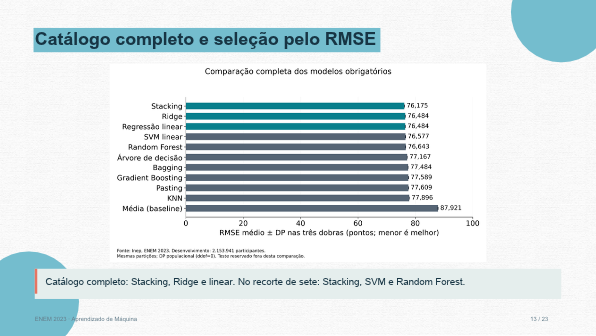
\includegraphics[height=3.5cm,trim=0 26.88bp 0 0,clip]{figuras/roteiro/slide-13.png}\end{center}
\rotulo{Fala principal sugerida}
No catálogo completo, o menor RMSE médio foi do Stacking, 76,175 pontos. Depois vêm Ridge e linear, ambos arredondados para 76,484. Antes do arredondamento, Ridge ficou ligeiramente à frente. No recorte de sete famílias, os três primeiros são Stacking, SVM linear e Random Forest. Essa diferença de escopo explica os dois trios apresentados durante o projeto. As buscas contemplaram a união deles: cinco modelos.
\rotulo{Explicação para estudar e aprofundar}
Os RMSE não arredondados são 76,174516 para Stacking, 76,483610 para Ridge e 76,483799 para linear. A escolha usa RMSE no desenvolvimento, não o resultado do teste. O gráfico inclui a média, com 87,921, e mostra dez regressores mais essa referência. As pequenas barras de erro representam o DP das dobras, não significância. KNN, Bagging, Pasting e Boosting foram avaliados, mas não ficaram no trio do recorte de sete. Não identificamos uma causa única para suas diferenças; elas dependem dos dados, da representação e das configurações testadas.
\rotulo{Como explicar o visual}
Leia o eixo horizontal e destaque que menor é melhor. Mostre as três primeiras linhas e depois explique o empate visual entre Ridge e linear.
\rotulo{Pergunta provável e resposta}
SVM e Random Forest são segundo e terceiro gerais? Não. Essa colocação vale apenas para o recorte de sete algoritmos.
\rotulo{Transição}
Também testamos se uma representação mais informativa das entradas reduziria o erro.
\vfill{\raggedright\scriptsize\color{navy} Conferência no projeto: resultados/comparacao\_modelos.csv; resultados/figuras/18\_comparacao\_completa.png.}\par
\clearpage
{\color{teal}\small SLIDE 14 / 23 - PAULO}\par
{\color{navy}\Large\bfseries Engenharia de atributos}\par
{\small Engenharia de atributos e regras usadas}\par
\begin{center}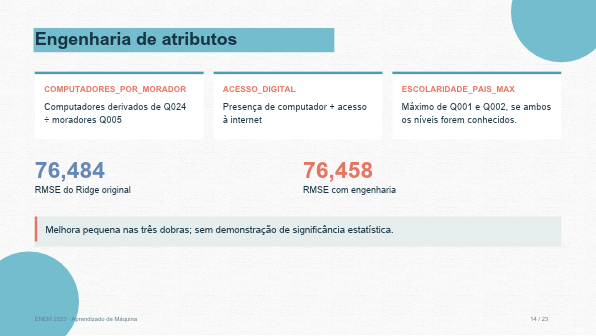
\includegraphics[height=3.5cm,trim=0 26.88bp 0 0,clip]{figuras/roteiro/slide-14.png}\end{center}
\rotulo{Fala principal sugerida}
Criamos três atributos derivados: computadores por morador, acesso digital e maior escolaridade dos responsáveis. O objetivo foi apresentar relações que poderiam ser úteis ao Ridge. O RMSE caiu de 76,484 na receita original para 76,458 com engenharia. A melhora é pequena e não foi submetida a teste de significância. Essa é uma comparação de representação, sem alterar o conjunto de participantes ou consultar o teste final.
\rotulo{Explicação para estudar e aprofundar}
Q024 é convertida de A a E para zero a quatro computadores; a última alternativa informa quatro ou mais, então quatro é um limite inferior. A divisão usa Q005 entre um e vinte moradores; fora disso, o atributo derivado fica ausente. Acesso digital soma presença de computador e internet, de zero a dois quando ambas são conhecidas. Escolaridade máxima mapeia A a G para níveis de zero a seis e exige as duas respostas conhecidas: desconhecimento não recebe nível inventado. O preenchimento posterior de ausências aprende somente no treino. Esse índice digital é uma construção operacional, não uma escala social validada.
\rotulo{Como explicar o visual}
Mostre as três fórmulas conceituais e a pequena redução do RMSE. Não apresente essa diferença como grande avanço.
\rotulo{Pergunta provável e resposta}
Criamos dados fictícios? Não. São transformações determinísticas de respostas reais, com regras explícitas e tratamento de desconhecimento.
\rotulo{Transição}
Em seguida, tentamos reduzir a quantidade de informações da representação.
\vfill{\raggedright\scriptsize\color{navy} Conferência no projeto: src/enem\_base/variants.py: ProfileFeatures.}\par
\clearpage
{\color{teal}\small SLIDE 15 / 23 - PAULO}\par
{\color{navy}\Large\bfseries Seleção de atributos e PCA}\par
{\small Seleção de atributos e PCA}\par
\begin{center}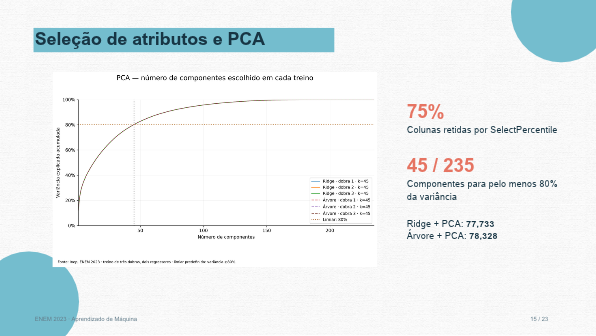
\includegraphics[height=3.5cm,trim=0 26.88bp 0 0,clip]{figuras/roteiro/slide-15.png}\end{center}
\rotulo{Fala principal sugerida}
Testamos duas estratégias diferentes de redução. A seleção manteve 75\% das colunas codificadas após a engenharia, escolhidas pelo teste F de regressão. O PCA criou componentes que preservam pelo menos 80\% da variância. Nas receitas avaliadas, nenhuma estratégia melhorou o erro global. O PCA reteve 45 componentes de uma representação original de 235 dimensões, tanto no Ridge quanto na árvore.
\rotulo{Explicação para estudar e aprofundar}
Selecionar mantém um subconjunto de colunas existentes; PCA cria novas combinações numéricas delas. Preservar variância significa conservar dispersão das entradas, não necessariamente informação útil para prever a nota. Por isso, compressão não garante menor RMSE. O Ridge com seleção teve 76,529. Com PCA, o Ridge passou de 76,484 para 77,733 e a árvore de 77,167 para 78,328. Houve seis ajustes de PCA: dois regressores em três dobras, sempre aprendendo os componentes no treino. A seleção foi experimentada no Ridge. A receita final vencedora não utiliza PCA.
\rotulo{Como explicar o visual}
No gráfico, o eixo horizontal é o número de componentes e o vertical é a variância acumulada. Mostre o cruzamento do limiar de 80\% em 45 componentes.
\rotulo{Pergunta provável e resposta}
O que são as 235 dimensões? São colunas da representação após preparação, principalmente indicadores categóricos; não são 235 perguntas originais.
\rotulo{Transição}
Também investigamos o equilíbrio das notas e a contribuição de blocos de atributos.
\vfill{\raggedright\scriptsize\color{navy} Conferência no projeto: src/enem\_base/variants.py: VariancePCA e SelectPercentile.}\par
\clearpage
{\color{teal}\small SLIDE 16 / 23 - PAULO}\par
{\color{navy}\Large\bfseries Ponderação e duas ablações}\par
{\small Ponderação e ablações}\par
\begin{center}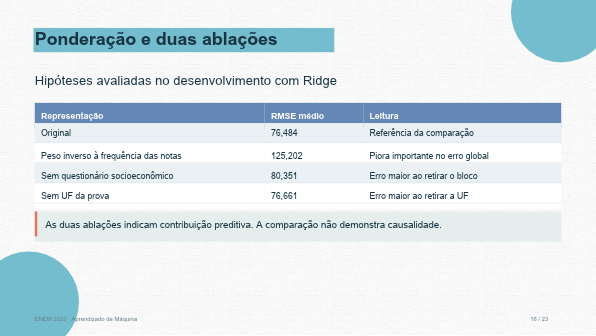
\includegraphics[height=3.5cm,trim=0 26.88bp 0 0,clip]{figuras/roteiro/slide-16.png}\end{center}
\rotulo{Fala principal sugerida}
A ponderação deu mais peso às faixas de notas menos frequentes durante o treino. O RMSE global do Ridge piorou para 125,202. Também fizemos duas ablações: retirar o questionário socioeconômico elevou o RMSE para 80,351; retirar a UF da prova elevou para 76,661. Esses resultados mostram que as propostas precisam ser medidas: uma mudança aparentemente razoável pode prejudicar o critério global.
\rotulo{Explicação para estudar e aprofundar}
Os pesos são inversos à frequência de dez faixas de largura igual, calculadas a partir do alvo do treino. Eles alteram a importância de exemplos no ajuste, sem criar participantes. A avaliação global continua usando o mesmo RMSE para permitir comparação. Ablação é retirar um bloco e observar a mudança, mantendo o protocolo. O aumento do erro sugere contribuição preditiva dessas entradas nessa configuração, mas não identifica efeito causal. Não treinamos um modelo separado para cada renda ou UF. Uma melhoria de alguma faixa não basta para declarar melhora do resultado global.
\rotulo{Como explicar o visual}
Compare cada linha à receita original de 76,484. Destaque o resultado negativo da ponderação e explique por que ele também é um achado.
\rotulo{Pergunta provável e resposta}
Isso prova que renda determina a nota? Não. Mostra contribuição preditiva do bloco socioeconômico nas condições observadas.
\rotulo{Transição}
Depois da representação, avaliamos alternativas de hiperparâmetros.
\vfill{\raggedright\scriptsize\color{navy} Conferência no projeto: src/enem\_base/variants.py: TrainingWeightedRegressor;\\ resultados/tabelas/comparacoes\_cv\_completas.csv.}\par
\clearpage
{\color{teal}\small SLIDE 17 / 23 - PAULO}\par
{\color{navy}\Large\bfseries Busca de hiperparâmetros}\par
{\small Busca de hiperparâmetros e congelamento}\par
\begin{center}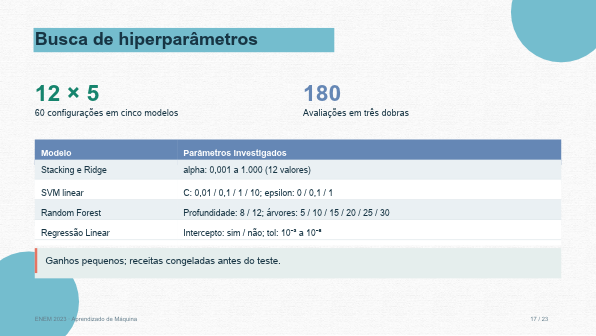
\includegraphics[height=3.5cm,trim=0 26.88bp 0 0,clip]{figuras/roteiro/slide-17.png}\end{center}
\rotulo{Fala principal sugerida}
Hiperparâmetros são escolhas que definimos antes de ajustar o modelo, como profundidade, quantidade de árvores ou força da regularização. Testamos doze configurações em cada um de cinco modelos: sessenta configurações e cento e oitenta avaliações nas três dobras. A decisão usou o RMSE do desenvolvimento. Os ganhos foram mínimos, e as receitas foram congeladas antes de abrir o teste final.
\rotulo{Explicação para estudar e aprofundar}
GridSearchCV avalia combinações de uma grade, usando as partições persistidas via PredefinedSplit. Stacking e Ridge variaram alpha; a SVM variou C e epsilon; a floresta variou profundidade e número de árvores; a linear variou intercepto e tolerância. Na busca da SVM, max\_iter foi ampliado para 50.000; isso não deve ser confundido com a configuração inicial de 5.000. O Stacking selecionou alpha=1000, Ridge alpha=10 e linear tol=1e-5. SVM e floresta mantiveram as receitas iniciais. A linear de referência levada ao teste mantém tol=1e-6. A tolerância numérica de decisão não é teste de significância.
\rotulo{Como explicar o visual}
Leia 12 por 5 e depois multiplique pelas três dobras. Evite chamar as 180 avaliações de 180 algoritmos diferentes.
\rotulo{Pergunta provável e resposta}
Parâmetro aprendido e hiperparâmetro são iguais? Não. Coeficientes são aprendidos no ajuste; alpha e profundidade são escolhas da configuração.
\rotulo{Transição}
As curvas ajudam a entender o comportamento das receitas com quantidades crescentes de treino.
\vfill{\raggedright\scriptsize\color{navy} Conferência no projeto: src/enem\_base/tuning.py: MODELS e SPACES; resultados/tabelas/antes\_depois.csv.}\par
\clearpage
{\color{teal}\small SLIDE 18 / 23 - PAULO}\par
{\color{navy}\Large\bfseries Curvas de aprendizado dos três modelos}\par
{\small Leitura das curvas de aprendizado}\par
\begin{center}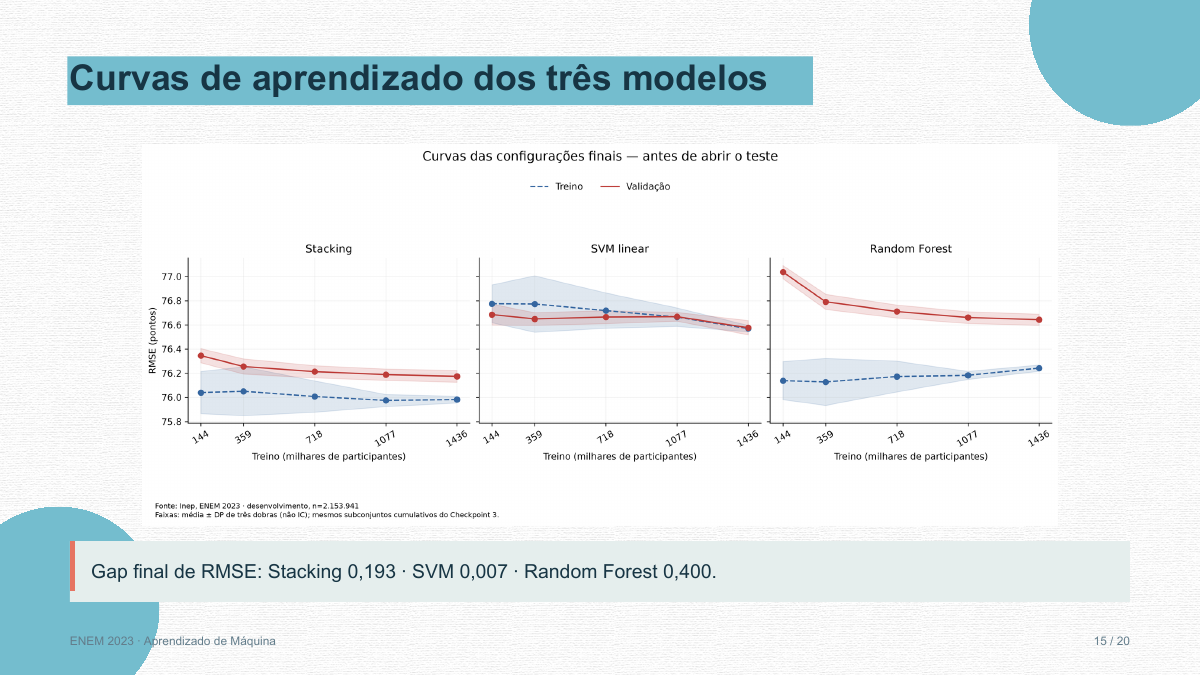
\includegraphics[height=3.5cm,trim=0 64.81bp 0 0,clip]{figuras/roteiro/slide-18.png}\end{center}
\rotulo{Fala principal sugerida}
As curvas mostram o erro de treino e de validação quando usamos 10\%, 25\%, 50\%, 75\% e 100\% do treino de cada dobra. A validação permanece fixa. Nos três modelos, as curvas finais ficam próximas, com diferenças de RMSE de 0,193 no Stacking, 0,007 na SVM e 0,400 na floresta. Isso não sugere sobreajuste acentuado nessas condições, mas não comprova desempenho em outra edição do ENEM.
\rotulo{Explicação para estudar e aprofundar}
O eixo horizontal indica quantidade de participantes de treino e o vertical indica RMSE. Cada ponto resume três dobras. Sobreajuste costuma produzir erro de treino muito menor que validação; subajuste pode aparecer quando o modelo não captura padrões úteis nem no treino. Gap pequeno, sozinho, não garante um modelo adequado ou ausência absoluta de sobreajuste. O menor treino já tem cerca de 143.596 participantes. Existem 45 pontos iniciais e 45 finais, com reuso registrado: trinta pontos iguais de SVM/floresta, doze do Stacking com bases reutilizadas e novo combinador, e três vindos das buscas em treino completo.
\rotulo{Como explicar o visual}
Aponte primeiro a legenda treino/validação, depois a distância entre as linhas e o efeito de aumentar os dados. As faixas mostram DP, não intervalo de confiança.
\rotulo{Pergunta provável e resposta}
São noventa treinamentos novos? Não. São pontos registrados, parte deles obtida com reuso compatível de ajustes ou bases.
\rotulo{Transição}
Com a receita congelada, chegamos à avaliação final separada.
\vfill{\raggedright\scriptsize\color{navy} Conferência no projeto: resultados/tabelas/curvas\_resumo.csv; src/enem\_base/frozen\_curves.py.}\par
\clearpage
{\color{teal}\small SLIDE 19 / 23 - PAULO}\par
{\color{navy}\Large\bfseries Teste final em 538.486 participantes}\par
{\small Teste final e relevância do resultado}\par
\begin{center}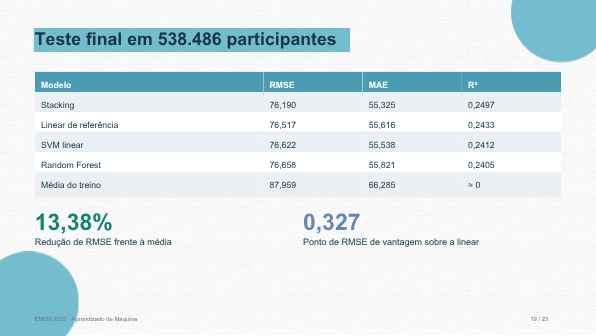
\includegraphics[height=3.5cm,trim=0 26.88bp 0 0,clip]{figuras/roteiro/slide-19.png}\end{center}
\rotulo{Fala principal sugerida}
No teste de 538.486 participantes, o Stacking teve RMSE de 76,190, MAE de 55,325 e R\textsuperscript{2} de 0,2497. A regressão linear ficou próxima, com RMSE de 76,517. SVM e floresta tiveram 76,622 e 76,658. A média teve 87,959. A redução do RMSE do Stacking frente à média foi de 13,38\%; a vantagem frente à linear foi de apenas 0,327 ponto. Isso exige uma interpretação equilibrada.
\rotulo{Explicação para estudar e aprofundar}
Os cinco modelos foram ajustados no desenvolvimento completo, com receitas previamente definidas, e avaliados nos mesmos IDs do teste. A seleção veio do desenvolvimento; não voltamos a escolher parâmetros após consultar o teste. A presença da linear e da média permite avaliar alternativas simples. Ridge, árvore, KNN, Bagging, Pasting e Boosting têm CV completa, mas não previsões nesse teste final. O R\textsuperscript{2} indica redução do erro quadrático frente à variação em torno da média observada, não percentual de pessoas acertadas. Os tempos de ajuste observados foram 1.250,63 s para Stacking e 36,41 s para linear; não constituem benchmark isolado de hardware.
\rotulo{Como explicar o visual}
Leia a tabela por RMSE, depois use MAE e R\textsuperscript{2} para complementar. Mostre que o ganho de 13,38\% se refere à média, não à regressão linear.
\rotulo{Pergunta provável e resposta}
O vencedor é estatisticamente superior? Não fizemos teste de significância. Podemos afirmar que apresentou o menor RMSE observado neste protocolo.
\rotulo{Transição}
A média global do erro não revela onde as previsões falham mais.
\vfill{\raggedright\scriptsize\color{navy} Conferência no projeto: resultados/tabelas/comparacao\_teste.csv; src/enem\_base/final\_evaluation.py.}\par
\clearpage
{\color{teal}\small SLIDE 20 / 23 - PAULO}\par
{\color{navy}\Large\bfseries Erros concentrados nos extremos}\par
{\small Diagnóstico dos extremos e resíduos}\par
\begin{center}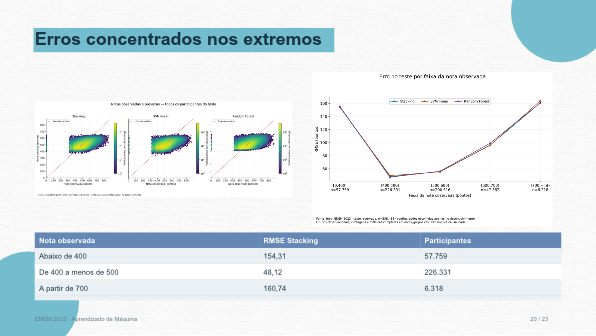
\includegraphics[height=3.5cm,trim=0 26.88bp 0 0,clip]{figuras/roteiro/slide-20.png}\end{center}
\rotulo{Fala principal sugerida}
No observado versus previsto, a diagonal representa previsão perfeita. As estimativas se concentram mais no centro da escala: notas baixas tendem a ser superestimadas e notas altas, subestimadas. No Stacking, o RMSE foi 154,31 abaixo de quatrocentos pontos e 160,74 a partir de setecentos. Entre quatrocentos e menos de quinhentos, ficou em 48,12. Portanto, o desempenho global esconde uma dificuldade importante nos extremos.
\rotulo{Explicação para estudar e aprofundar}
As células coloridas agregam todos os participantes do teste, sem substituir a base por uma amostra de pontos. O gráfico por faixa usa a nota observada para agrupar o diagnóstico depois da previsão, não como entrada do modelo. Há 57.759 participantes abaixo de 400, 226.331 em [400,500) e 6.318 a partir de 700. Resíduo é observado menos previsto: negativo indica superestimação; positivo, subestimação. Os resíduos médios do Stacking foram -118,60 e +156,03 nas faixas extremas. Resíduo médio e RMSE são medidas diferentes: o primeiro conserva o sinal; o segundo mede magnitude.
\rotulo{Como explicar o visual}
Explique a diagonal e o significado das cores antes de interpretar a concentração central. Depois conecte os extremos do gráfico às linhas da tabela.
\rotulo{Pergunta provável e resposta}
O modelo acerta todo mundo com erro de 76 pontos? Não. RMSE é um resumo agregado; erros individuais e por faixa podem ser muito maiores.
\rotulo{Transição}
Também verificamos como os erros se distribuem entre grupos de participantes.
\vfill{\raggedright\scriptsize\color{navy} Conferência no projeto: resultados/figuras/11\_observado\_previsto.png; resultados/tabelas/erros\_grupos.csv.}\par
\clearpage
{\color{teal}\small SLIDE 21 / 23 - PAULO}\par
{\color{navy}\Large\bfseries Análise por grupos de participantes}\par
{\small Grupos de escola, renda e UF}\par
\begin{center}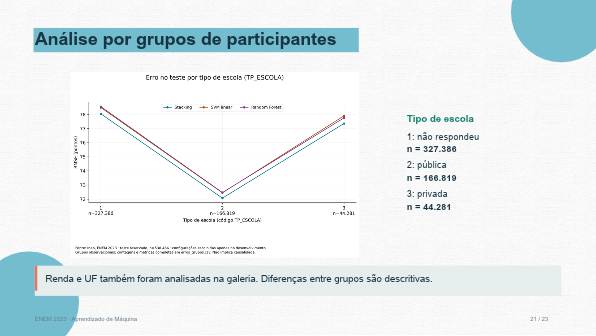
\includegraphics[height=3.5cm,trim=0 26.88bp 0 0,clip]{figuras/roteiro/slide-21.png}\end{center}
\rotulo{Fala principal sugerida}
O gráfico compara erros por tipo de escola, sem treinar modelos diferentes para cada grupo. Temos 327.386 participantes que não responderam essa informação, 166.819 de escola pública e 44.281 de escola privada. As contagens são importantes porque os grupos têm tamanhos e perfis diferentes. Também analisamos renda e UF de aplicação. Essas diferenças são diagnósticos descritivos de previsão, sem demonstrar causalidade.
\rotulo{Explicação para estudar e aprofundar}
O eixo vertical representa RMSE, não a média das notas e nem a qualidade da escola. Um grupo com erro menor não pode ser apresentado automaticamente como mais capaz ou melhor atendido pelo sistema educacional. As características e a distribuição das notas podem variar entre grupos. O código 1 de TP\_ESCOLA é uma alternativa própria de não resposta, que não foi fundida com escola pública ou privada. SG\_UF\_PROVA descreve aplicação, não necessariamente residência. Renda Q006 é autodeclarada. Os erros de renda e UF e suas contagens estão nas figuras e tabelas do projeto; não exibimos resultados fictícios no slide.
\rotulo{Como explicar o visual}
Mostre a legenda dos modelos, o RMSE e os tamanhos dos grupos. Reforce que o gráfico mede erro de previsão, e não ranking de desempenho escolar.
\rotulo{Pergunta provável e resposta}
A análise comprova justiça do modelo? Não. Diferenças descritivas de RMSE, isoladamente, não certificam equidade nem adequação a decisões individuais.
\rotulo{Transição}
Esses diagnósticos ajudam a delimitar o que podemos concluir.
\vfill{\raggedright\scriptsize\color{navy} Conferência no projeto: resultados/figuras/14\_escola.png; 15\_uf.png; 16\_renda.png; resultados/tabelas/erros\_grupos.csv.}\par
\clearpage
{\color{teal}\small SLIDE 22 / 23 - PAULO}\par
{\color{navy}\Large\bfseries Limites e rastreabilidade}\par
{\small Evidências, testes e limites}\par
\begin{center}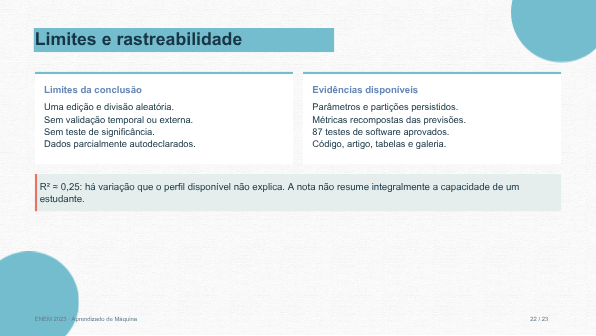
\includegraphics[height=3.5cm,trim=0 26.88bp 0 0,clip]{figuras/roteiro/slide-22.png}\end{center}
\rotulo{Fala principal sugerida}
Preservamos parâmetros, partições, métricas e evidências de execução para permitir conferência. A suíte atual teve 87 testes de software aprovados. Esses testes verificam o código e não são novas rodadas de treinamento nacional. Cientificamente, analisamos uma edição e uma divisão aleatória. Não fizemos validação temporal, avaliação externa ou teste de significância entre modelos. O R\textsuperscript{2} perto de 0,25 mostra que o perfil disponível não captura toda a variação da nota.
\rotulo{Explicação para estudar e aprofundar}
As comparações iniciais têm 33 avaliações por dobra; as variantes somam 21. As buscas têm 180 avaliações e as curvas incluem reuso documentado. O teste final reúne cinco modelos. Não some tudo como se cada registro fosse um ajuste novo. Dados fictícios ficam isolados nos testes de software; treinamento nacional e métricas científicas utilizam participantes reais. Os agregados e o código estão no repositório; arquivos individuais grandes são locais. A divisão fixa e os hashes apoiam rastreabilidade, mas não garantem reprodução bit a bit em qualquer ambiente ou generalização para outro ano. Respostas autodeclaradas e ausências também limitam a análise.
\rotulo{Como explicar o visual}
Separe as duas colunas: limites científicos e evidências técnicas. A aprovação de testes de código não elimina os limites da pesquisa.
\rotulo{Pergunta provável e resposta}
Os 87 testes provam que o modelo generaliza? Não. Generalização é avaliada por dados separados; os testes de software verificam contratos e comportamento da implementação.
\rotulo{Transição}
Encerramos com a contribuição demonstrada e as próximas perguntas de pesquisa.
\vfill{\raggedright\scriptsize\color{navy} Conferência no projeto: tests/; resultados/manifesto\_entrega.json; README.md.}\par
\clearpage
{\color{teal}\small SLIDE 23 / 23 - PAULO}\par
{\color{navy}\Large\bfseries Conclusões e próximos passos}\par
{\small Conclusão e encerramento do pitch}\par
\begin{center}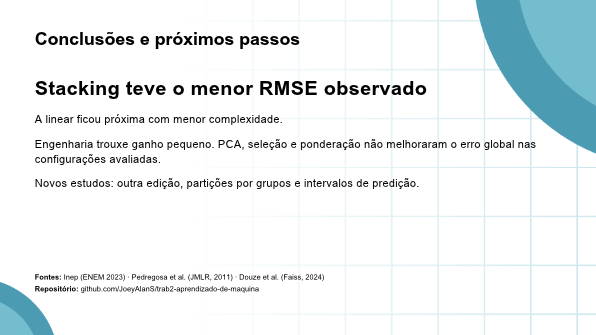
\includegraphics[height=3.5cm,trim=0 26.81bp 0 0,clip]{figuras/roteiro/slide-23.png}\end{center}
\rotulo{Fala principal sugerida}
Concluímos que o Stacking apresentou o menor RMSE observado, mas a regressão linear foi uma alternativa muito próxima e mais simples. A engenharia teve ganho pequeno; PCA, seleção e ponderação não melhoraram o erro global nas configurações avaliadas. Nossa contribuição é uma comparação nacional documentada, incluindo os limites e as hipóteses que não funcionaram. Os próximos estudos são outra edição, partições por grupos e intervalos de predição. Essas etapas futuras ainda não foram realizadas.
\rotulo{Explicação para estudar e aprofundar}
Ao defender o resultado, diferencie vantagem observada de superioridade universal. O custo adicional do Stacking e a pequena distância para a linear precisam ser considerados junto das métricas. A execução nacional demonstrou viabilidade computacional no ambiente do estudo, mas não foi avaliada como serviço em produção nem como solução de impacto educacional. A nota não resume a capacidade de um estudante. A mensagem final pode ser: comparamos métodos de forma consistente, medimos os erros reais e identificamos o alcance e os limites das previsões.
\rotulo{Como explicar o visual}
Retome a pergunta do slide 2 e a resposta sustentada pelas métricas. Aponte as fontes e encerre abrindo espaço para perguntas.
\rotulo{Pergunta provável e resposta}
Qual seria o próximo passo mais importante? Avaliar uma receita previamente definida em outra edição ou divisão por grupos, para testar estabilidade além desta partição.
\rotulo{Transição}
Obrigado. Ficamos à disposição para explicar as escolhas, os resultados e os limites do estudo.
\vfill{\raggedright\scriptsize\color{navy} Conferência no projeto: docs/artigo.md; README.md; referências do artigo.}\par
\end{document}
